%! suppress = MissingLabel

% Preamble
\documentclass[a4paper]{article}

\usepackage{geometry}
\geometry{
    a4paper,
    scale=0.8,
    bottom=2cm,
    top=2cm,
}

% Packages
\usepackage{amsmath}
\usepackage{csquotes}
\usepackage{natbib}
\usepackage{blindtext}
\usepackage{ctex}

\usepackage[utf8]{inputenc}
\usepackage[english]{babel}
\usepackage{indentfirst}
\usepackage{enumitem}
\usepackage{floatrow}
\usepackage{graphicx}
\usepackage{amsfonts}
\usepackage{amssymb}
\usepackage{listings}

% set up BNF generator
\usepackage{syntax}
\setlength{\grammarparsep}{10pt plus 1pt minus 1pt}
\setlength{\grammarindent}{10em}


\setlist{noitemsep} % removes spacing from items but leaves space around the whole list
%\setlist{nosep} % removes all vertical spacing within and around the list
\setlist[itemize]{topsep=0.25em, leftmargin=1.5pc}
\setlist[enumerate]{topsep=0.25em, leftmargin=1.5pc}

\renewcommand{\baselinestretch}{1.2}

%\setlength{\parindent}{0em}
\graphicspath{ {./} }

%! suppress = EscapeUnderscore
\newcommand*{\tproject}[1]{
    \begin{math}
        \pi_{#1}
    \end{math}
}

%! suppress = EscapeUnderscore
\newcommand*{\tselect}[1]{
    \begin{math}
        \sigma_{#1}
    \end{math}
}

\newcommand{\emptyline}{\\ \hspace*{\fill} \\}

\newcommand*{\textbfit}[1]{\textbf{\textit{#1}}}

\newcommand*{\seqdef}[1][a]{$({#1}_n)_{n\geq1}$}
\newcommand*{\subseqdef}[1][a]{$({{#1}_n}_i)_{i\geq1}$}
\newcommand*{\seq}[1][a]{#1_n}
\newcommand*{\limtoinf}[1][n]{\lim_{#1\rightarrow\infty}}
\newcommand{\abs}[1]{\left| #1 \right|}

\newcommand{\shell}[1]{\lstinline!#1!}
\usepackage{sourcecodepro}
\usepackage[T1]{fontenc}

\usepackage{hyperref}
\usepackage{xcolor}
\usepackage{textcomp}
\hypersetup{
    colorlinks,
    linkcolor={blue!50!black},
    citecolor={blue!50!black},
    urlcolor={blue!80!black}
}

\lstset{breaklines=true,basicstyle=\ttfamily\small,autogobble=true,language=C}

% Document
%! suppress = TooLargeSection
%! suppress = Quote
\begin{document}
    \title{
        \vspace{-3em}
        Human Centred Design Techniques Portfolio}
    \author{
        Group 43
    }
    \date{\vspace{-2em}}
    \maketitle

    \subsection*{The Problem}

    Jay, a computing student at Imperial College, is currently studying for his exams.
    He encountered a problem and attempted to get assistance from his friends, but they could not reach an agreement.
    Subsequently, he turned to Edstem, the school’s forum, to post a thread.
    Despite his expectation for a response from the tutors, he was left unanswered.
    Alice, on the other hand, is a finance student from the LSE. She enjoys expressing her thoughts, but her lack of confidence inhibits her from posting responses publicly on the school forum.
    Moreover, she holds the belief that the tutors' responses are generally more authoritative.
    Thus, even when she could potentially provide useful insights to some questions, she often holds back, allowing the tutors to take the lead.

    From a tutor's perspective, the lack of responses is not by choice but a matter of necessity.
    Philip, a Graduate Teaching Assistant at UCL, explained, ``I simply don't have enough time to respond to all posts, let alone provide immediate replies.''

    The existing school forum presents challenges; it neither guarantees students will receive responses nor fosters an environment for them to share ideas.
    Furthermore, it places undue pressure on the tutors.

    In our quest for solutions, we discovered that peer discussions could be vital.
    More frequent peer discussions could minimize the need for students to post questions persistently to obtain answers.
    Moreover, with more participants engaging in the discussion, a broader spectrum of ideas can be collected, leading to more comprehensive outcomes.
    This approach could not only decrease the workload of the tutors, but also establish social connections within academic community, as there are more peer interactions.


    Hence, we aim to develop a student-centric platform that encourages peer discussions.
    By ensuring users receive sufficient feedback and promoting confidence to respond to questions, we aim to cultivate a more collaborative learning environment.
    We tried to figure out: How might we promote peer discussions of exercise solutions among college students to minimize the effort they need to review and validate solutions,
    while reducing the workload of tutors and building networks within academic community.

    \section*{Testing and Validation}

    \subsection*{Concept and Initial Design}
    \begin{minipage}{0.4\textwidth}
        \centering
        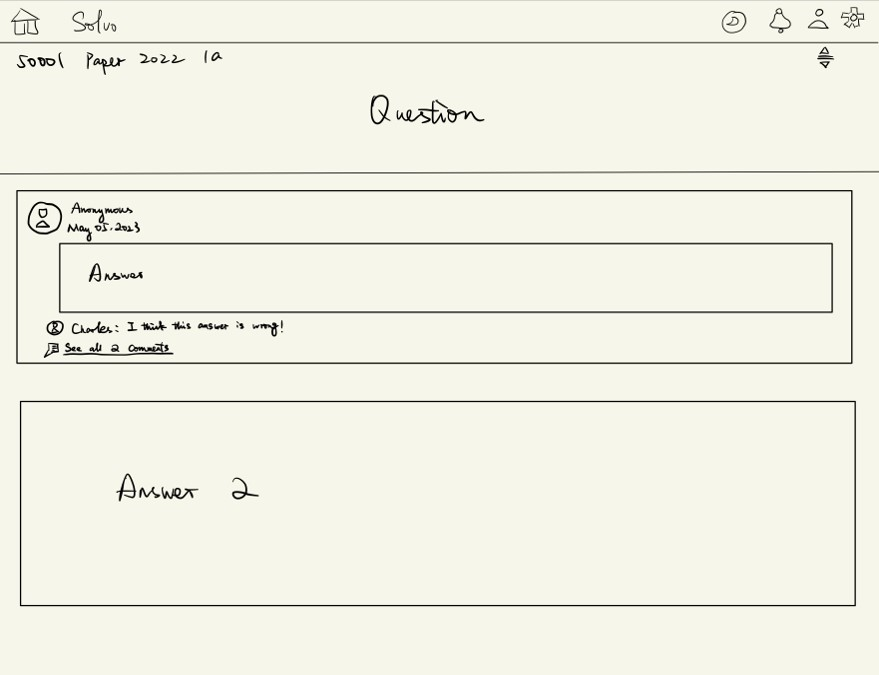
\includegraphics[width=\textwidth]{concept2}
        \captionof{}{Question page: concept}
    \end{minipage}\hspace{0.05\textwidth}
    \begin{minipage}{0.57\textwidth}
        \centering
        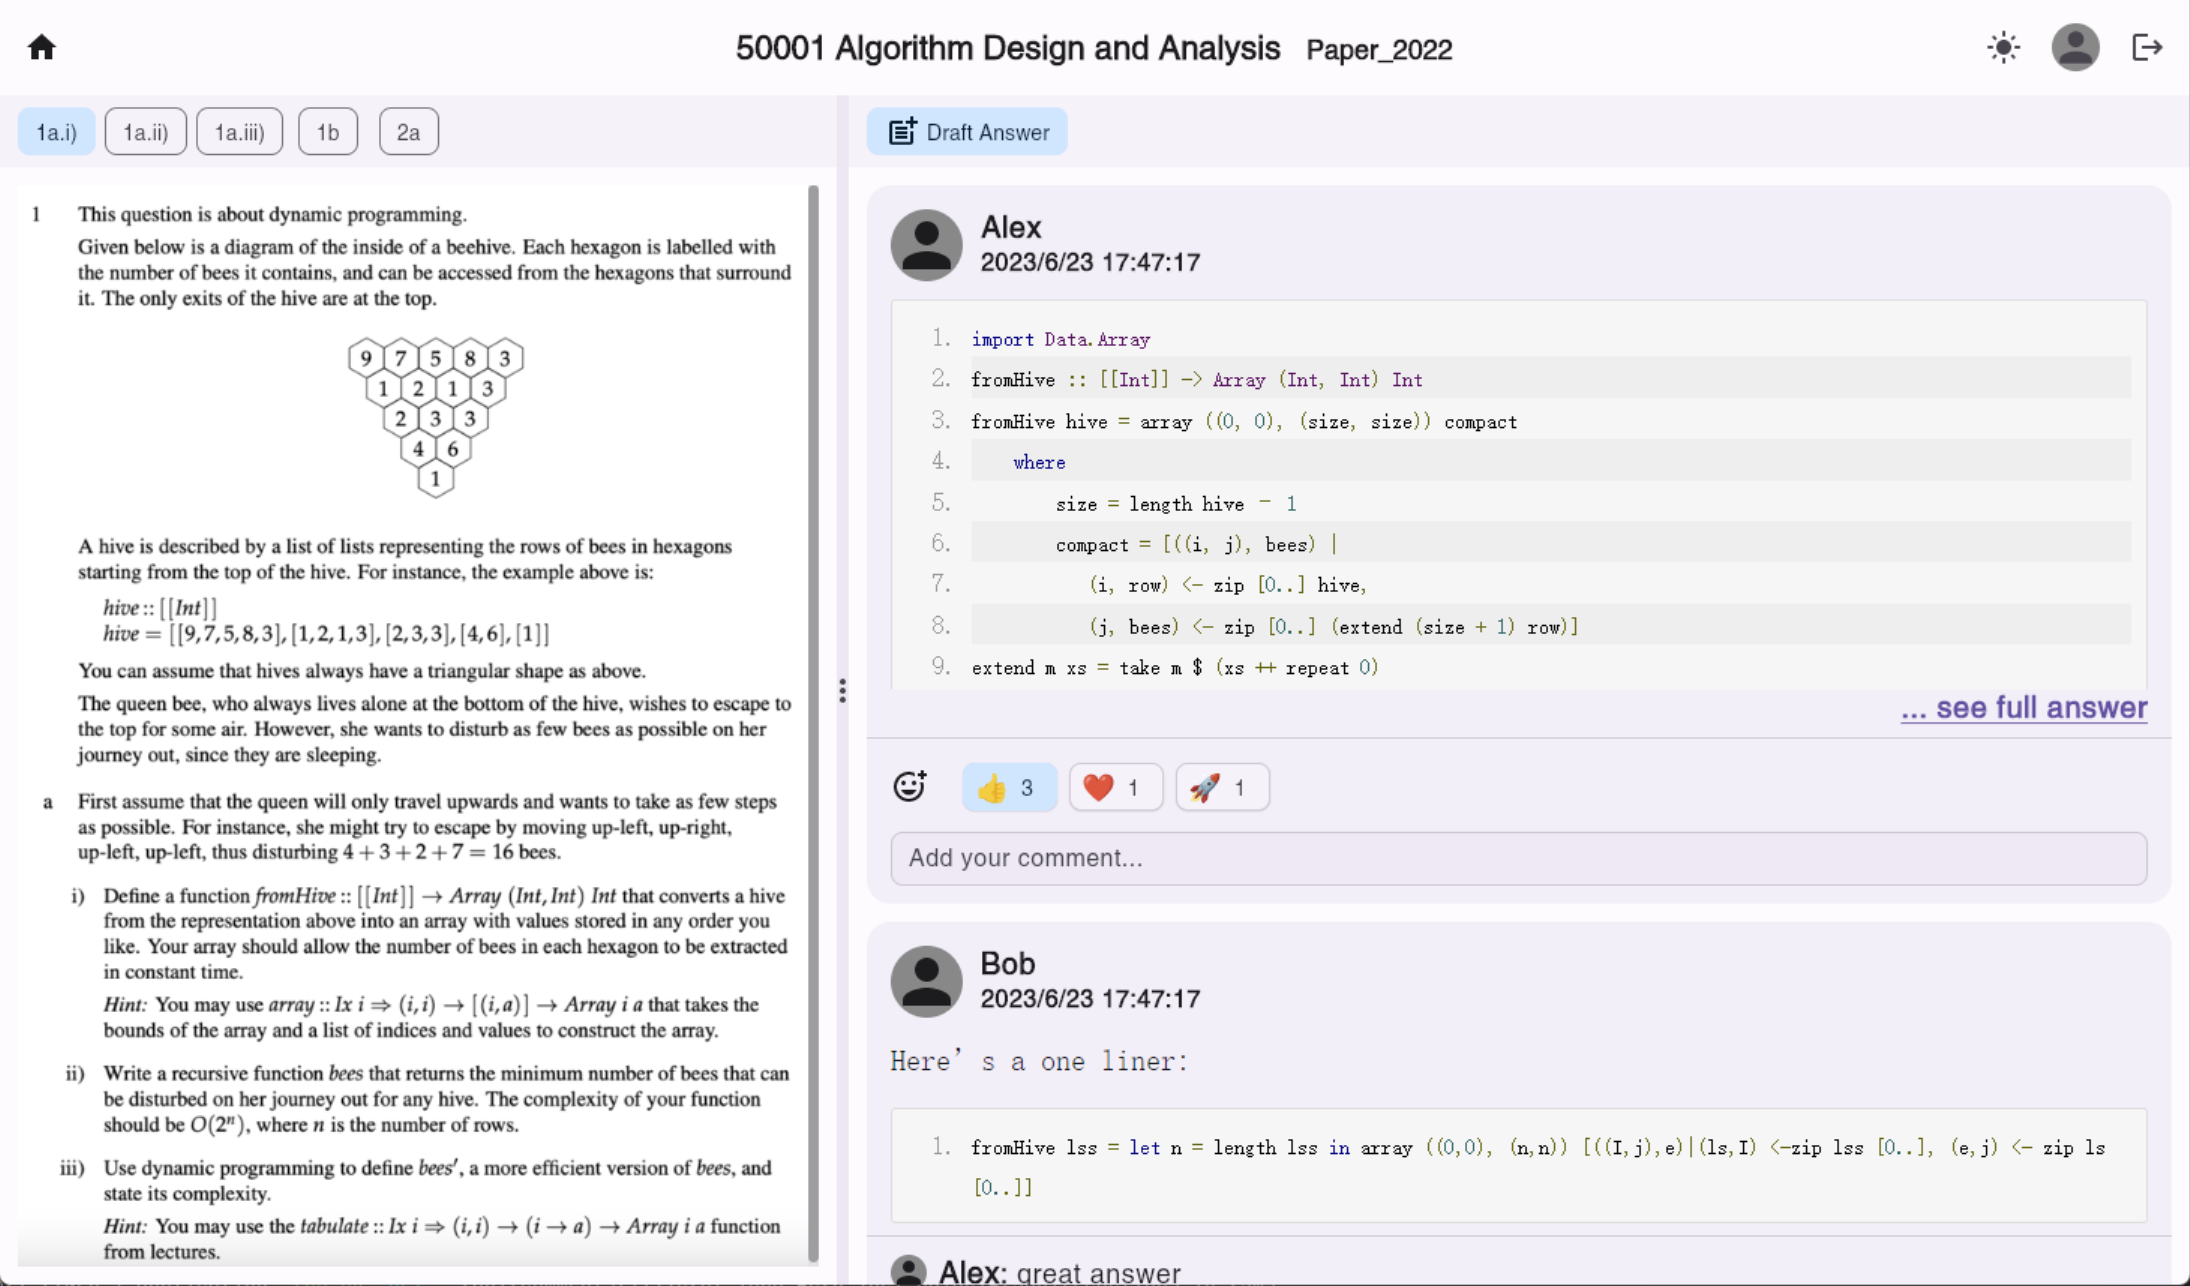
\includegraphics[width=\textwidth]{question-page2}
        \captionof{}{Initial design}
    \end{minipage}
    \\
    \begin{minipage}{0.4\textwidth}
        \centering
        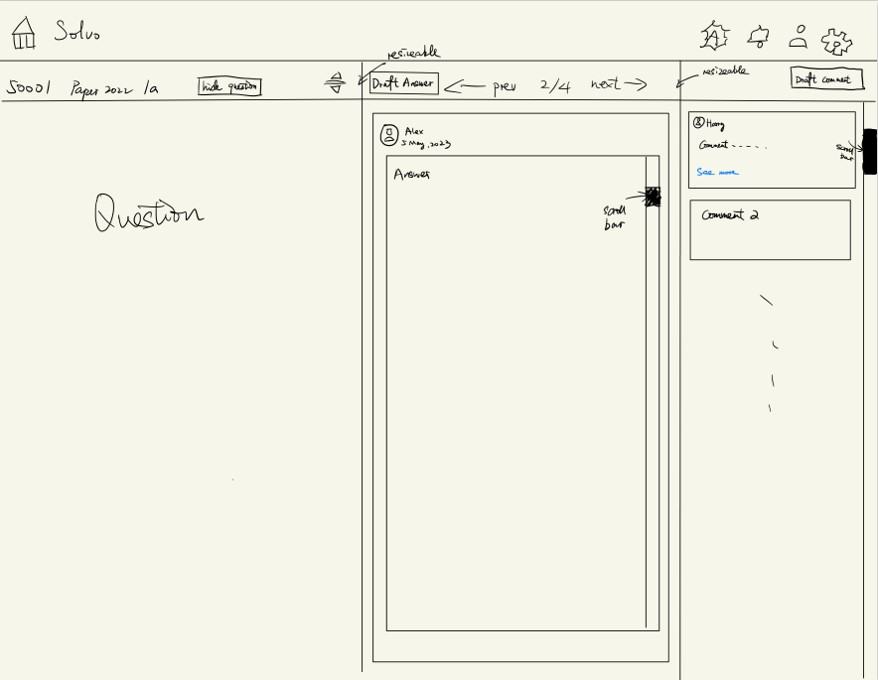
\includegraphics[width=\textwidth]{concept1}
        \captionof{}{Comment page: concept}
    \end{minipage}\hspace{0.05\textwidth}
    \begin{minipage}{0.57\textwidth}
        \centering
        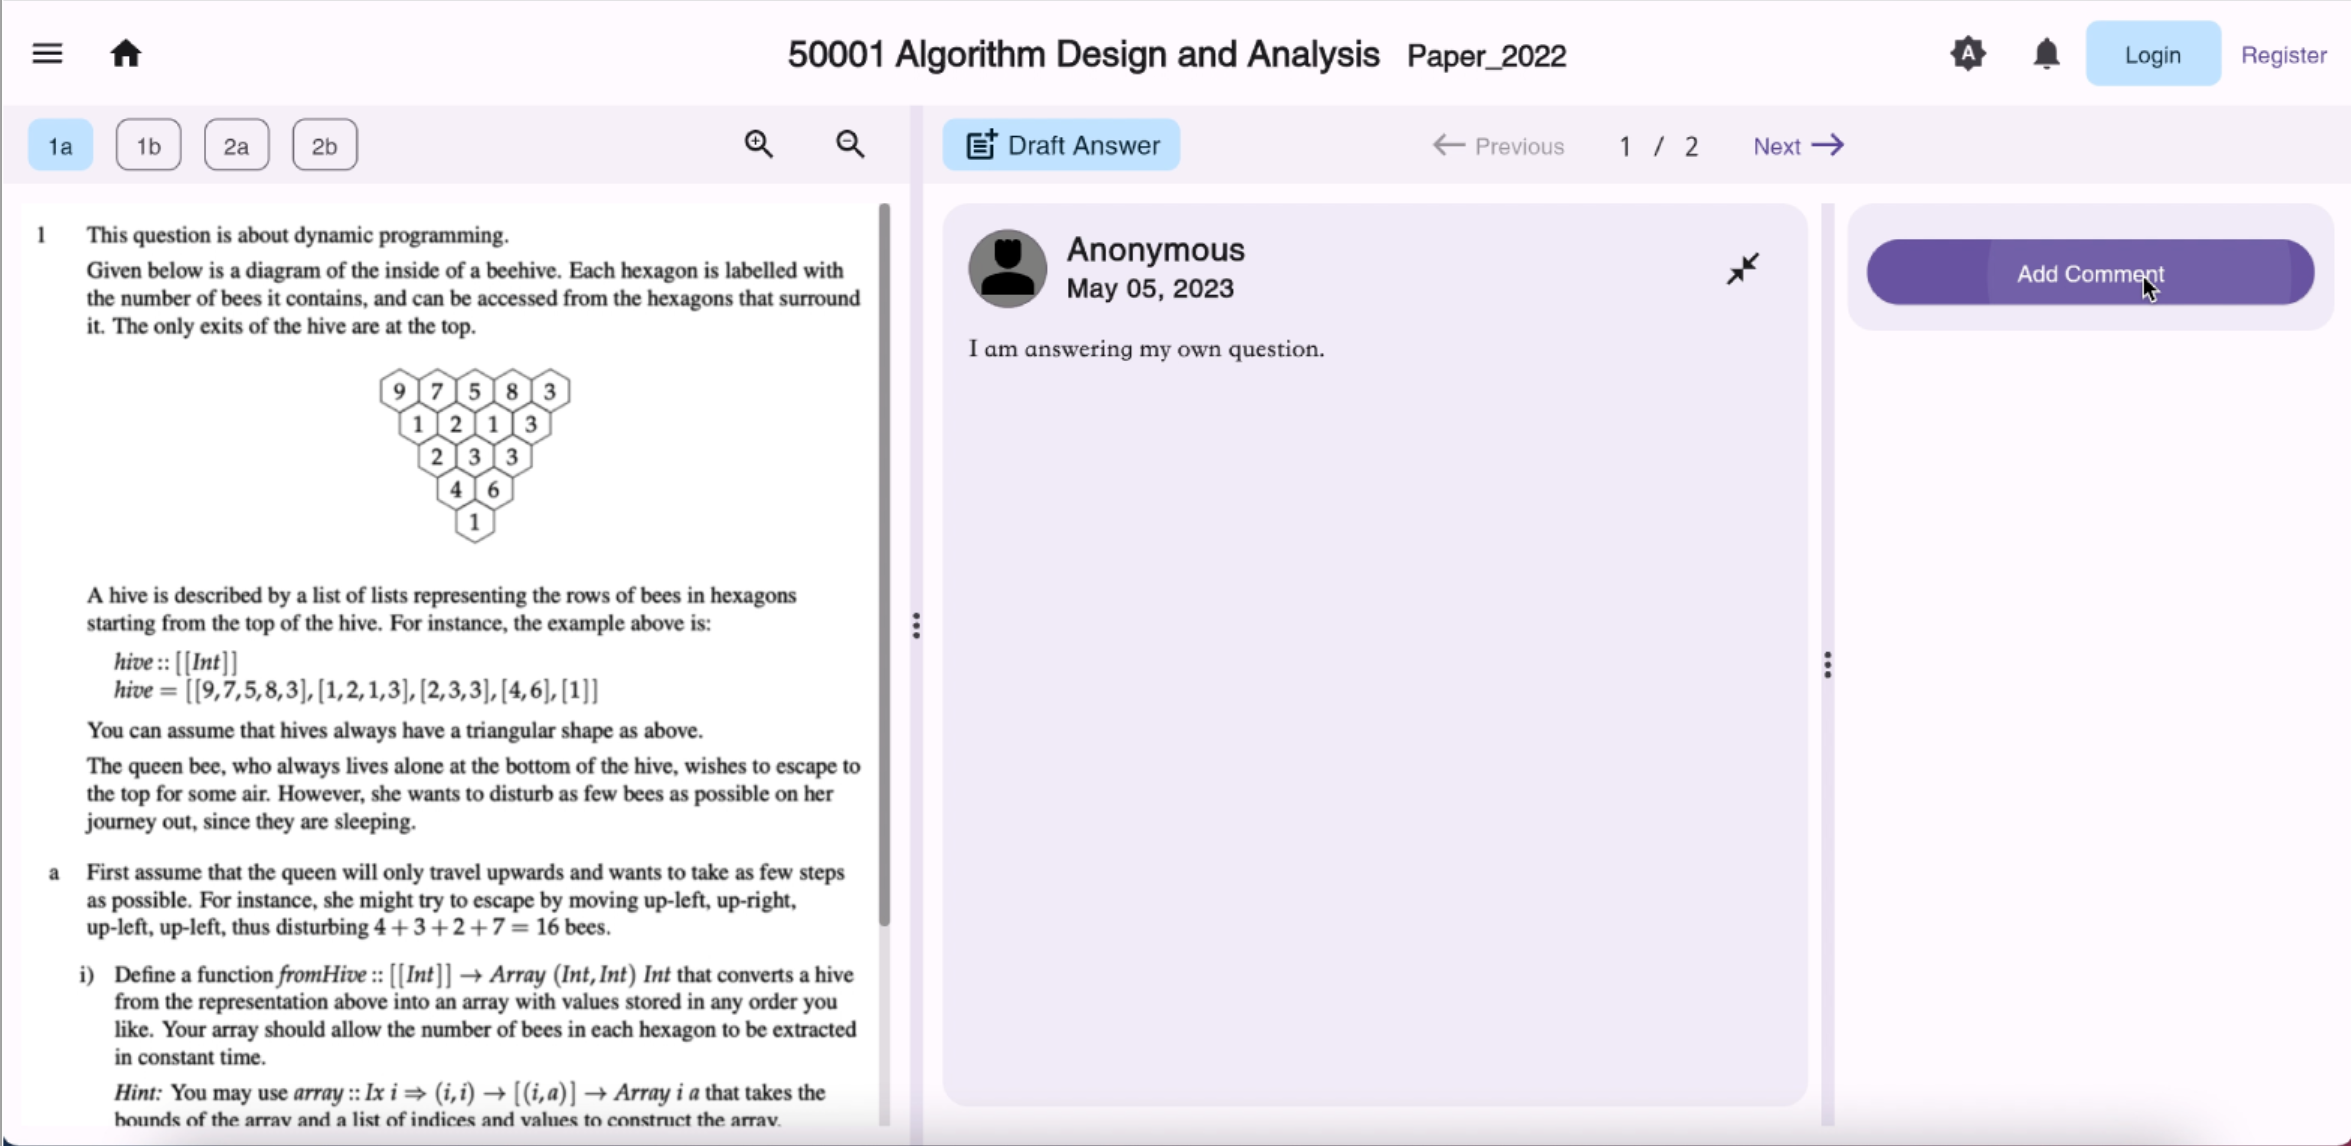
\includegraphics[width=\textwidth]{question-page1}
        \captionof{}{Initial design}
    \end{minipage}

    \subsection*{Reaction System}
    \subsubsection*{Motivation}
    Users reflects that they are sometimes reluctant to post comments because:
    \begin{itemize}
        \item[-] ``Although sometimes I do feel like to leave some words, I'm just too lazy to think of the sentence and to type it out.''
        \item[-] ``Sometimes I want to express my agreement for someone's answer, but I think the comment area are for those thoughtful opinions,
                 not for something like `you're right' `plus 1', so I would choose not to say anything.''
        \item[-] ``I am too shy to post my opinions at public platforms.
                   It's better if you could have an anonymous system.''
    \end{itemize}
    To summarize, users tend to be lazy to type long comments, while short and less meaningful comments like ``you're right'' seem to not quite fit into the comment area for some users.
    Some of them might be shy to post contents if we do not support anonymous posting.

    So our goal is to provide another way for users to give feedback to others, which is lighter and more convenient to use than comments, and is better to be anonymous.

    \subsubsection*{Design}
    A Reaction system is designed allowing viewers to quickly give feedback to answers by simply clicking on a button with emojis, instead of composing a text comment.
    The number of different emoji reactions received will be displayed at the bottom of the answer box.

    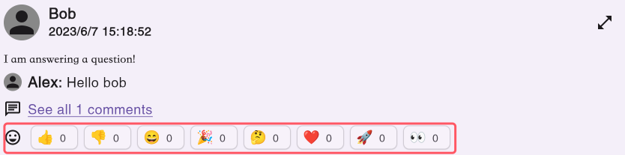
\includegraphics{reaction}

    \subsubsection*{Feedbacks and Reflection}
    We bring the design to users for validation, and most users agree that the feature makes them more motivated to give feedback to other's answers.
    \begin{itemize}
        \item[-] ``This is exactly what I want when I feel agreed with someone - without this I wouldn't want to post a comment.
                   If I disagree with someone, though, I would probably click thumbs down and then post a comment explaining my ideas.''
        \item[-] ``As a person who posts answers, I would love to see feedbacks given in this way because these emojis are really straight forward and self-explanatory.
                   It also provides diversity of the kind of feedbacks I can receive.''
    \end{itemize}
    The feature encourages users to give feedbacks to other's answers by providing a system that is easy to use and understand,
    and it could also benefit the ones who post answers because they can receive larger quantity of and more diverse feedbacks in this way.
    Therefore, it stimulates peer discussion on our platform, which is what we're targeting to achieve.

    \subsubsection*{Digital Touch-point Evolution}
    (Image: Question page with reaction system)

    \subsection*{Thoughts}

    \iffalse
    \subsubsection*{Motivation}
    \subsubsection*{Design}
    \subsubsection*{Feedbacks and Reflection}
    \subsubsection*{Digital Touch-point Evolution}
    \fi

    \subsection*{Edit, Delete and Anonymous}

    \iffalse
    \subsubsection*{Motivation}
    \subsubsection*{Design}
    \subsubsection*{Feedbacks and Reflection}
    \subsubsection*{Digital Touch-point Evolution}
    \fi

    \subsection*{Papers Upload}

    \iffalse
    \subsubsection*{Motivation}
    \subsubsection*{Design}
    \subsubsection*{Feedbacks and Reflection}
    \subsubsection*{Digital Touch-point Evolution}
    \fi

    \section*{Impacts}

    \subsection*{Impact for Target Audience}

    Interviews were conducted to understand how Solvo can affect the stakeholders.

    We came back to students who used to discuss only with friends.
    The users responded with the following quotes:
    \begin{itemize}
        \item \textit{``Do you think you would be willing to use it if you understood this feature (the thoughts)?''}
        \begin{itemize}
            \item[-] ``Yeah, if I only have some general ideas, I will definitely not post an answer.
            But if I know that I can post `Thoughts', I am glad to share them.''
        \end{itemize}

        \item \textit{``Do you think you will be getting more feedback with the reaction system?''}
        \begin{itemize}
            \item[-] ``Sure.''
            \item[-] ``For me, I will write a comment only when I think the answer is incorrect.
            If I agree with the answer, I won't say `You are correct', which takes time.''
        \end{itemize}

        \item
        \textit{``As a user, are you willing to give more feedback using the reaction system?''}
        \begin{itemize}
            \item[-] ``Yeah absolutely.''
            \item[-] ``I don’t want the comments to be filled up with meaningless comments like `+1'.
            With this reaction system, it can be much more clean.''
        \end{itemize}
        \item \ldots
    \end{itemize}

    As it can be summarized from the quotes:

    On Solvo, students who used to discuss only with friends can now share ideas with more people, and receive feedback from peers.
    Students can therefore gain feedback from the reactions and comments, knowing if they are appreciated by others,
    and learn what they can't learn in the past.

    \subsection*{Impact for Other Stakeholders}

    We interviewed five tutors about their thoughts on Solvo.

    \begin{itemize}
        \item \textit{``Will you welcome your institution to introduce Solvo to students?''}
        \begin{itemize}
            \item[-] ``Of course.''
            \item[-] ``I love the peer discussion it (Solvo) provides.
            As a tutor, we always encourage students to discuss with each other and answer questions on the forum, even if it might be wrong.
            This allows them to learn from each other.''
        \end{itemize}
    \end{itemize}

    It is known from the interviews that tutors like the way Solvo promotes peer discussion, and are happy to welcome the introduction of Solvo.

    These connections can extend beyond the classroom and may lead to collaborations, study groups, or professional relationships that continue throughout their university experience and beyond.
\end{document}
